% vim: set spelllang=fr:
\chapter{Annotation en rôles sémantiques fondée sur la connaissance}
\label{ch:srl}

%\citep{simmons1973semantic} is the earliest work on Semantic Role Labeling.
%Already based on \citep{fillmore1968case}, it parsed a sentence into what we
% know call semantic roles. (check)

%Contrairement aux autres ressources pour l'annotation en rôles sémantiques,
%VerbNet couvre l'ensemble des verbes fréquents du vocabulaire tout en étant
%conçu sur des préceptes robustes le rendant utile pour les tâches de Traitement
%Automatique des Langues (Section~\ref{ch:verbnet:sec:verbnet}).

La tâche d'annotation en rôles sémantiques a reçu beaucoup d'attention ces
dernières années, à la fois pour les approches supervisées et semi-supervisées.
Les approches fondées sur la connaissance, elles, ne se basent pas sur des
corpus annotés mais sur des ressources lexicales existantes. Ce type d'approche
a été négligé malgré leur complémentarité par rapport aux autres approches.

En nous inspirant de \cite{swier2004unsupervised,swier2005exploiting}, nous
présentons dans ce chapitre un système d'annotation en rôles sémantiques fondé
sur la connaissance qui se veut simple à mettre en place et facile à
reproduire. La prise en compte de divers phénomènes linguistiques doit
permettre d'améliorer les performances. Par exemple, la prise en compte de la
voix passive a réduit le taux d'erreur de 15,7~\%, ce qui montre la marge de
progrès existante. Malgré des performances moindres par rapport aux approches
supervisées quand des données d'entraînement existent, l'approche facilite
l'analyse des erreurs, n'a pas besoin d'un corpus annoté manuellement et est
\textit{a priori} indépendante du domaine considéré, étant donné qu'elle
utilise le lexique VerbNet.

Ce chapitre se concentre sur notre système d'annotation en rôles sémantiques
dans un cadre général en l'utilisant sur le corpus FrameNet anglais (qui a été
présenté à la section~\ref{presentation_framenet}). Le
Chapitre~\ref{ch:domainsrl} montrera la versatilité de ce système dans des
contextes différents :
\begin{itemize}
    \item en domaine spécifique avec les domaines du football, du
réchauffement climatique et de l'informatique,
    \item et dans deux langues différentes : anglais et français.
\end{itemize}

Le travail présenté dans ce chapitre a été réalisé en collaboration avec
Guilhem Pujol durant son stage d'ingénieur. Ce chapitre est une réécriture
complète de travaux pour la plupart déjà publiés \citep{pradet2013revisiting}.

\section{Tâche}

L'objectif de ce chapitre est d'annoter en rôles sémantiques le corpus
FrameNet, largement utilisé pour l'évaluation
\citep{baker2007semeval,das2010probabilistic}. Nous souhaitons cependant
l'évaluer en utilisant la ressource VerbNet. Pour ce faire, nous utilisons le
projet SemLink \citep{bonial2012empirically} qui propose un mapping de rôles
sémantiques entre les frames FrameNet et les classes VerbNet ce qui permet
d'évaluer l'annotation en rôles sémantiques VerbNet sur FrameNet.

La Figure~\ref{fig:srlrussia} est un exemple d'annotation en rôles sémantiques
avec des frames et des rôles FrameNet. Nous utiliserons notamment cette phrase
d'exemple par la suite pour illustrer notre propos. Pour une phrase donnée, les
prédicats verbaux (\textit{trigger} ou déclencheur dans la terminologie FrameNet)
et la frame qu'ils évoquent sont identifiés. Dans chaque phrase, des syntagmes
vont remplir un des rôles prévus par la frame dans FrameNet. Ces syntagmes sont
nommés «~remplisseurs de rôle~» (\textit{role filler} en anglais). L'analyse
est locale : seule la phrase courante est considérée.

\begin{figure}[t]
    La phrase à annoter est :

    \begin{quote}
    However, in 2002 Russia declared it will eliminate its tactical nuclear weapons by the end of 2004.
    \end{quote}

    L'objectif est d'aboutir à la représentation suivante :

    \begin{itemize}
        \item \textit{declare} déclenche la frame Statement dont les rôles sont remplis ainsi :
        \begin{itemize}
            \item Speaker : Russia
            \item Message : it will eliminate its tactical nuclear weapons by the end of 2004
            \item Time : in 2002
        \end{itemize}
        \item \textit{eliminate} déclenche la frame Removing dont les rôles sont remplis ainsi :
        \begin{itemize}
            \item Agent: it
            \item Theme: its tactical nuclear weapons
            \item Source: \textit{non instancié}
        \end{itemize}
    \end{itemize}
    \caption{\label{fig:srlrussia}Exemple d'annotation en rôles sémantiques. Le
    vocabulaire FrameNet est ici utilisé (voir la
section~\ref{vocverbnetframenet}).}

\end{figure}

Toute interprétation supplémentaire non présente dans la
Figure~\ref{fig:srlrussia} est en dehors du cadre de l'annotation en rôles
sémantiques, ce qui est la raison pour laquelle la tâche est aussi connue sous
le nom d'analyse sémantique de surface (\textit{shallow semantic parsing}). Il
est néanmoins important de garder à l'esprit les applications possibles de tels
travaux. Par exemple, un système de question-réponse pourrait utiliser la
représentation de ces deux \textit{frames} pour répondre à la question
\textit{Does Russia possess tactical nuclear weapons?} L'annotation de la
Figure~\ref{fig:srlrussia} est une information utile, mais elle ne serait pas
suffisante pour répondre à la question : il faut aussi comprendre la question,
annoter les coréférences (\textit{it} fait référence à \textit{Russia}),
comprendre la sémantique de \textit{Removing}, établir la crédibilité du
\textit{Speaker}, s'intéresser à d'autres phrases potentiellement
contradictoires, etc.

\section{Système}

Le système que nous présentons est une implémentation améliorée et libre du
système décrit par \cite{swier2004unsupervised,swier2005exploiting}. Les
ressources utilisées ont beaucoup progressé (VerbNet 1.5 contre VerbNet 3.2
notamment). Les corpus sur lesquels s'évaluer ont aussi évolué. En particulier,
les systèmes basés sur FrameNet n'utilisent plus le corpus de phrases
d'exemples choisis pour leur diversité syntaxique mais s'évaluent sur des
annotations de toutes les frames présentes dans des textes issus de différentes
sources. \cite{swier2005exploiting} utilisent aussi un mapping non disponible
alors que le projet SemLink a fourni un mapping FrameNet-VerbNet «~officiel~».
Dix ans après, il est donc important d'évaluer à nouveau cette approche pour
savoir où elle se situe par rapport à l'état de l'art. Nous proposons par
ailleurs certaines améliorations.

Pour commencer, chaque phrase à annoter doit d'abord être étiquetée en
morphosyntaxe et analysée syntaxiquement. Nous laissons ici ces analyses à des
systèmes externes présentés à la section~\ref{subsec:details_exp}. Ces analyses
sont l'entrée de notre système, la sortie étant l'annotation en rôles
sémantiques montrée dans la Figure~\ref{fig:srlrussia}.

Ensuite, nous utilisons les informations de VerbNet (présenté à la
section~\ref{presentation_verbnet}) sur l'interface entre la syntaxe et la
sémantique. Dans VerbNet, chaque classe regroupe un certain nombre de verbes
acceptant tous les mêmes constructions syntaxiques. Les syntagmes participant à
ces constructions sont associés à des rôles sémantiques à interpréter dans le
contexte de la classe. Ces \textit{frames} sont notées de cette façon :
NP.Agent V NP.Theme. Ici, dans cette construction transitive (NP V NP, e.g.
\textit{Sally pushed the chair}), le premier syntagme nominal (\textit{Sally})
est Agent alors que le second (\textit{the chair}) est Theme.  Bien que des
règles précises régissent leur attributions, l'interprétation complète des
rôles (ici Theme et Agent) dépend de la classe VerbNet considérée. Par exemple,
la classe \texttt{resign-10.11} contient la frame NP.Agent V PP.Source
(\textit{I resigned from the military}). Dans cette classe, l'Agent est la
personne qui démissionne et la Source est le poste qui a été quitté.

Pour une phrase donnée, le système commence par identifier les verbes de cette
phrase. Pour chacun de ces verbes, un ensemble de classes VerbNet est
identifié. Ainsi, pour notre phrase d'exemple ci-dessus, les classes possibles
pour le verbe \textit{declare} sont \texttt{declare-29-4-1-1-1},
\texttt{say-37.7-1} et \texttt{reflexive\_appearance-48.1.2}. Le choix correct
est \texttt{say-37.7-1}, mais il ne nous est pas possible de le déterminer
avant de considérer les frames listées par VerbNet dans ces différentes
classes.

Par exemple, \texttt{reflexive\_appearance-48.1.2} contient la frame NP.Agent V
NP.Theme. Ainsi, si un des verbes de cette classe, tel que \textit{present} :
\begin{itemize}
    \item est utilisé dans un sens compatible avec la classe
        \texttt{reflexive\_appearance-48.1.2},
    \item et est utilisé avec un sujet syntagme nominal et un objet syntagme
        nominal,
\end{itemize}
alors le sujet du verbe est l'Agent et l'objet est le Theme, ce que des
applications pourront interpréter dans le contexte de la classe VerbNet
\texttt{reflexive\_appearance-48.1.1}.

La phrase d'exemple de la Figure~\ref{fig:srlrussia} ne correspond pas à NP V
NP mais à NP V that S (\textit{that S} étant la notation VerbNet pour les
complétives introduites par \textit{that}). La seule occurrence de cette frame
VerbNet est dans \texttt{say-37.7-1} : NP.Agent V that S.Topic (\textit{He
ordered that he go}). Les classes \texttt{declare-29-4-1-1-1} et
\texttt{reflexive\_appearance-48.1.2} ne listant pas cette frame, il est
possible d'établir que :

\begin{itemize}
    \item la classe VerbNet qui convient est \texttt{say-37.7-1},
    \item \textit{Russia} est Agent,
    \item \textit{it will eliminate its tactical nuclear weapons by the end of 2004} est Topic.
\end{itemize}

Enfin, le mapping de VerbNet vers FrameNet (section~\ref{subsec:mapping}) nous
informe que :

\begin{itemize}
    \item la classe VerbNet \texttt{say-37.7} correspond à la frame Statement,
    \item dans cette classe, le rôle VerbNet Agent correspond au rôle FrameNet Speaker,
    \item dans cette classe, le rôle VerbNet Topic correspond au rôle FrameNet Topic.
\end{itemize}

Nous aboutissons ainsi à l'annotation en rôles sémantiques voulue pour notre
phrase d'exemple.

On ne peut pas toujours identifier la classe VerbNet correcte. C'est le cas par
exemple de \texttt{reflexive\_appearance-48.1.2} et \texttt{say-37.7-1} qui
contiennent toutes les deux le cadre NP V NP. Ainsi, si notre phrase d'exemple
avait été \textit{Russia declared its intentions}, la classe serait restée
ambigüe. Sans corpus annoté, ces ambiguïtés ne peuvent pas être résolues.
Cependant, une fois qu'une première série de correspondances a été effectuée,
il est possible d'utiliser les connaissances du domaine étudié pour annoter de
nouveaux syntagmes nominaux (section~\ref{subsec:probability}).

Alors que nous avons jusqu'ici décrit le principe général du système afin d'en
donner l'intuition, les sections suivantes expliquent le fonctionnement précis
du système qui est découpé en quatre étapes.

\subsection{Identification du prédicat}

Chaque phrase peut contenir un ou plusieurs prédicats : nous nous contentons
ici de retenir tous les verbes présents dans VerbNet. Les autres prédicats
potentiels, c'est-à-dire ceux qui ne sont pas dans VerbNet et ne sont pas des
verbes, sont ignorés. Les parties du discours acceptées sont toutes celles
concernant des verbes simples : MD, VB, VBD, VBG, VBN, VBP,
VBZ\footnote{FrameNet annonce utiliser simplement les parties du discours des
    ressources utilisées \citep[section~3.1]{ruppenhofer2006extended}, mais
    cela semble correspondre au tagset du TreeTagger.}. Les autres formes où le
    verbe est composé de plusieurs mots (par exemple \textit{He has (VHZ)
    suffered (VVN) from loneliness}) ne sont pas actuellement prises en compte.

\subsection{Identification des arguments}
\label{argid}

Cette étape identifie les syntagmes amenés à jouer un rôle sémantique lors de
l'annotation. C'est un problème difficile ; la première raison est que seuls
78~\% des arguments du corpus FrameNet sont effectivement des sous-arbres issus
de l'analyse syntaxique. Nous suivons ici \cite{lang2011unsupervised} qui
propose huit règles\footnote{La septième règle n'est pas utilisée étant donné
    que nous ne prenons pas en compte les prédicats verbaux consistués de
plusieurs mots.} basées sur l'analyse syntaxique de la phrase. Initialement,
tous les mots sont candidats. Puis chacune de ces règles sélectionne ou écarte
des mots candidats. Dans la représentation en dépendances, si le mot
sélectionné est la tête d'un syntagme, c'est le syntagme entier qui devient
candidat. Sinon, c'est uniquement le mot.  Voici les règles appliquées dans
l'ordre :

\begin{enumerate}
    \item Éliminer les déterminants, les marqueurs d'infinitifs, les conjonctions de coordinations et la ponctuation.
    \item Éliminer les candidats dont le chemin du prédicat au candidat finit par une coordination, une subordination, etc.
    \item Conserver les candidats qui sont les sujets les plus proches à gauche du prédicat et dont les relations du prédicat p à la tête t du candidat sont toutes montantes (t $\rightarrow$ p).
    \item Éliminer les candidats  dont le chemin entre le prédicat et le candidat, sauf la dernière relation, contient une relation de sujet, une relation de modifieur adjectival, etc.
    \item Éliminer les verbes auxiliaires.
    \item Conserver les candidats directement sous le prédicat.
    \item \sout{Conserver les candidats si le chemin du prédicat au candidat traverse plusieurs noeuds verbaux.}
    \item Éliminer tous les candidats restants.
\end{enumerate}

Pour les règles 2 et 4, la liste complète des relations acceptées est donnée en
annexe à la section~\ref{argument_identification}. En pratique, sur le corpus
FrameNet, ces règles génèrent les candidats valides mais aussi certains qui ne
jouent pas de rôle. Grâce à la ressource VerbNet, notre système devra écarter
ces candidats, ce qui n'est pas nécessairement possible avec de simples
heuristiques.

\subsection{Utilisation des arguments de la vérité-terrain}

Nous évaluons notre système de deux manières :
\begin{itemize}
    \item avec les arguments identifiés automatiquement (section~\ref{argid}),
    \item et avec les arguments issus de la vérité-terrain.
\end{itemize}

En effet, l'objectif est d'évaluer l'apport de VerbNet à la tâche de
l'annotation en rôles sémantiques. L'identification des arguments, bien qu'une
partie intégrante de tout système complet d'annotation en rôles sémantiques
\citep{das2010probabilistic}, ne fait pas partie de nos contributions.

Pour convertir les arguments de la vérité-terrain vers une frame VerbNet, nous
utilisons simplement la position de ces arguments dans la phrase. Par exemple,
si un syntagme nominal apparaît avant le verbe et un syntagme prépositionnel
apparaît après le verbe, la frame VerbNet devient NP V PP. Bien que cela
corresponde en général au véritable cadre de sous-catégorisation de la phrase,
ce n'est pas toujours le cas. Montrons-le avec deux exemples.

\begin{itemize}
    \item Pour \textit{Les déchets éliminés polluent} et le verbe
        \textit{éliminé}, la frame est NP V, alors qu'il aurait fallu V NP.
    \item \textit{Il dégage le ballon} et \textit{Il le dégage} produisent
        respectivement les cadres NP V NP et NP NP V. Cependant, \textit{le
        ballon} et \textit{le} doivent tous les deux être considérés comme un
        syntagme nominal rattaché au verbe avant de comparer le cadre de
        sous-catégorisation de la phrase à VerbNet.
\end{itemize}

Ainsi, même lorsque les arguments de la vérité-terrain sont utilisés, l'absence
de prise en compte de la syntaxe est pénalisant, ce qu'il faudra traiter lors
de futurs travaux.

\subsection{Correspondance exacte des frames}
\label{correspondance_exacte}

Cette étape associe zéro, un ou plusieurs rôles sémantiques à chaque syntagme
candidat identifié lors de l'étape précédente. Elle correspond au \textit{frame
matching} de \citet{swier2005exploiting}.

Nous incluons ici deux étapes traditionnellement séparées dans les systèmes
d'annotation en rôles sémantiques : l'identification des frames FrameNet puis
l'assignation de rôles aux arguments précédemment identifiés
\citep{gildea2002automatic,das2014frame}. Nous commençons par identifier les
frames VerbNet possibles pour restreindre au maximum le nombre de classes
VerbNet applicables, le but étant de n'en avoir qu'une. En effet, même si
toutes les classes VerbNet réutilisent les mêmes rôles, le sens précis d'un
rôle est déterminé par la classe. Il faut donc l'identifier.

Regardons comment se déroule cette étape. Premièrement, les syntagmes candidats
sont représentés au format VerbNet. Par exemple, si trois syntagmes nominaux
ont été identifiés comme arguments, dont un avant le verbe, la représentation
VerbNet de la phrase devient NP V NP NP. Si le troisième syntagme est un
syntagme prépositionnel introduit par \textit{in}, la représentation devient NP
V NP in NP, et ainsi de suite.

Ensuite, pour comparer la représentation VerbNet de la phrase aux frames
VerbNet, nous identifions toutes les classes VerbNet incluant le prédicat. Par
exemple, le prédicat \textit{classify} est présent dans deux classes VerbNet~:
\texttt{characterize-29.2} et \texttt{classify-29.10}. Les frames VerbNet
possibles sont~:

\begin{itemize}
    \item characterize-29.2
    \begin{itemize}
        \item NP.Agent V NP.Theme (as) S\_ING.Attribute
        \item NP.Agent V NP.Theme to be ADJ.Attribute
        \item NP.Agent V NP.Theme as PP.Attribute
    \end{itemize}
    \item classify-29.10
    \begin{itemize}
        \item NP.Agent V NP.Theme
        \item NP.Agent V NP.Theme as PP.Goal
        \item NP.Agent V NP.Theme in PP.Location
    \end{itemize}
\end{itemize}

% TODO commencer par la phrase d'exemple (declare ou eliminate)
Considérons la phrase \textit{The curator classified the artifacts}. La
représentation VerbNet de cette phrase est NP V NP, ce qui correspond au
NP.Agent V NP.Theme de la classe \texttt{classify-29.10}. On en déduit que
\textit{The curator} est Agent, et que \textit{the artifacts} est Theme. Cette
phrase est donc correctement annotée en rôles sémantiques VerbNet.

Prenons un autre example, cette fois tiré de FrameNet. La phrase \textit{The
company also classifies short and wide radius ruts according to their severity}
est transformée en NP V NP according PP. Dans ce cas, seuls les deux premiers
syntagmes peuvent être mis en correspondance avec les frames VerbNet listées
ci-dessus. Il n'y a pas de correspondance possible pour le troisième syntagme:
VerbNet n'encode pas \textit{according} comme une préposition possible alors que
\textit{in} et \textit{as} sont acceptées. De tels arguments non prévus pas VerbNet
ne sont pas annotés lors de cette étape. C'est ici un problème de couverture.
Les auteurs de VerbNet travaillent actuellement sur la couverture de la
ressource en ajoutant des informations syntaxiques et lexicales issues de très
larges corpus \citep{bonial2013expanding}. Le résultat de ces travaux n'est
cependant pas disponible dans la version 3.2 de VerbNet que nous utilisons. Ce
problème de couverture empêche d'assigner la classe VerbNet qui convient. Par
conséquent, même si on sait que quelle que soit la classe, le sujet serait
Agent et le premier objet Theme, cette information est difficilement
interprétable dans une application.

Dans les cas où différentes frames VerbNet sont possibles, le calcul de scores
de correspondances présentés par \cite{swier2004unsupervised} peut aider à
désambiguïser, notamment en éliminant les \textit{frames} comportant trop
d'arguments. Cela dit, de nombreux arguments restent ambigus : la suite de la
désambiguïsation est l'objet des sections~\ref{subsec:probability} et
~\ref{restrictions_selection}.

% TODO différents algorithmes de match
% TODO nouvel algorithme : oublier complètement l'ordre

%Une autre difficulté fréquente en français est l'ordre des objets du verbe.
%Prenons les phrases suivantes, inspirées de la classe \texttt{cut-21.1} :

%\begin{itemize}
%    \item \textit{Luc a découpé la photo dans le journal avec des ciseaux}
%    \item \textit{Luc a découpé avec des ciseaux la photo sa maison de vacances dans le journal de la commune de Lacanau}
%    \item\e Luc a découpé avec des ciseaux dans le journal la photo où il montre l'énorme poisson qu'il venaît de pêcher
%\end{itemize}


\subsection{Correspondance probabiliste des frames}
\label{subsec:probability}

Maintenant que les correspondances exactes ont étés identifiées, il reste d'une
part les correspondances impossibles et les correspondances ambigües pour
lesquelles plusieurs frames sont possibles. Alors que les correspondances
impossibles sont à corriger au niveau de la ressource VerbNet ou au niveau de
l'analyse syntaxique, nous pouvons utiliser les frames déjà mises en
correspondance pour désambiguïser les correspondances ambigües. La méthode, une
forme d'induction, reste non supervisée : bien que nous entraînions une forme
simple d'algorithme supervisé, nous le faisons sur des données qui sont
initialement non annotées.  En effet, elles sont simplement obtenues
automatiquement sur le corpus existant à l'aide de la correspondance exacte.
Nous faisons ici l'hypothèse qu'un corpus entier est à annoter, mais dans le
cas où l'annotation se ferait phrase par phrase, il serait possible
d'abandonner cette étape ou d'alimenter les classifieurs que nous utilisons au
fur et à mesure des annotations. Cette étape correspond aux \textit{probability
models} de \citet{swier2004unsupervised}.

L'apprentissage se fait sous la forme d'un simple classifieur statistique. Le
classifieur (issu de \cite{swier2004unsupervised}) assigne une probabilité aux
différents rôles possibles en s'aidant des rôles déjà identifiés.

$$ \text{rôle} = \arg\max_{\text{rôle}} p(\text{rôle} \vert \text{prédicat}, \text{fonction})$$

La fonction est la fonction grammaticale identifiée d'après l'analyse
syntaxique : si un syntagme apparaît avant le verbe, il est sujet, s'il est
après le verbe, et il est objet, et ainsi de suite. Les syntagmes
prépositionnels sont traités à part : la préposition qui introduit le syntagme
est considérée à part.

Ce classifieur utilise l'information du prédicat et la fonction grammaticale
détectée. Par exemple, dans notre corpus (section~\ref{subsec:details_exp}),
l'objet direct du verbe \textit{négliger} est le plus souvent \textit{Theme}. La
précision pour ce modèle est forte, mais il n'assigne des rôles que pour 40~\%
des arguments : dans les autres cas, nous ne disposons pas d'informations pour
cette paire (prédicat, fonction grammaticale).

Une procédure de \textit{bootstrap} reposant sur les mêmes principes a aussi
été implémentée en suivant \cite{swier2004unsupervised}.

\subsection{Désambiguïsation de la classe VerbNet}

Un autre classifieur est utilisé pour déterminer la classe VerbNet en fonction
du prédicat.  Cette tâche a été déjà étudiée indépendemment
\citep{abend2008supervised,brown2011verbnet,kawahara2014single}. En effet, les
distinctions de sens proposées par VerbNet sont prometteuses car elles ne sont
pas aussi fines que celles de WordNet, ce qui a posé beaucoup de difficultés en
désambiguïsation lexicale \citep[section 10.1]{navigli2009word}, notamment
parce que l'accord inter-annotateur reste faible en annotant un corpus avec les
sens de WordNet. Concernant la désambiguïsation de sens VerbNet,
\cite{abend2009unsupervised} montrent que l'adaptation au domaine biomédical
dégrade fortement les résultats, alors que leur corpus était constitué d'un
nombre important de verbes monosémiques.

En désambiguïsation lexicale, il est généralement difficile de battre la
\textit{baseline} du sens le plus fréquent. Par exemple, lors de la tâche de
désambiguïsation lexicale de SemEval-2007, seuls 25~\% des systèmes ont fait
mieux que cette baseline, et les meilleurs systèmes ont incorporé cette
information. Nous choisissons de rester pour l'instant dans la simplicité en
utilisant directement cette baseline :

$$ \text{classe} = \arg\max_{\text{classe}} p(\text{classe} \vert \text{prédicat}) $$

La désambiguïsation est cependant facilitée : l'ensemble des classes candidates
a été auparavant restreint par les correspondances exactes et probabilistes.

\section{Gestion de la voix passive}
\label{sec:passif}

Une analyse d'erreur a révélé que la voix passive était une source d'erreurs
importante dans l'analyse de notre corpus FrameNet. En effet, VerbNet n'encode
pas la voix passive qui est un phénomène syntaxique, et non un phénomène
lexical, car (pratiquement) tous les verbes anglais permettent le passif (ce
qui n'est pas le cas du français). C'est donc au moment de l'analyse syntaxique
que les sujets et objets syntaxiques, profonds ou non, doivent être identifiés
correctement. Pour annoter la phrase \textit{the artifacts were classified by the
curator} en rôles sémantiques, il est donc important de d'abord transformer la
phrase en \textit{the curator classified the artifacts} avant d'effectuer la
correspondance avec les frames VerbNet.

Les sujets et objets profonds ne sont pas encodés dans les corpus annotés en
syntaxe que nous utilisons (le Wall Street Journal pour l'anglais, cf.
section~\ref{subsec:details_exp}). Une étape intermédiaire est donc nécessaire
entre l'analyse syntaxique et l'annotation en rôles sémantiques
\citep{bonfante2011modular, ribeyre2013systeme}. Cette étape intermédiaire
pourra identifier les sujets et objets profonds de tous les verbes considérés,
évitant ainsi toute une classe d'erreurs lors de l'annotation en rôles
sémantiques. 

Afin de valider cette hypothèse, nous nous sommes concentrés sur la voix
passive qui était le phénomène de syntaxe profonde le plus présent dans notre
corpus.  Pour annoter les verbes repérés comme étant utilisés avec la voix
passive (et uniquement pour ceux là), nous avons remplacé les frames VerbNet
par leur deux équivalents à la voix passive. Les verbes utilisés au passif en
anglais sont au participe passé et gouvernés par une forme du verbe \textit{to
be}. Étant donné une frame VerbNet telle que \textit{NP.Agent V NP.Theme (eg.
the curator classified the artifacts)}, nous la remplaçons par deux nouvelles
frames :

\begin{itemize}
    \item NP.Recipient V (the artifacts were classified)
    \item NP.Recipient V by NP.Agent (the artifacts were classified by the curator)
\end{itemize}

Ce sont ces frames VerbNet transformées qui sont utilisées lorsque qu'une voix
passive est detectée, ce qui améliore les résultats
(Table~\ref{table:results}). Cette expérience valide la gestion de tels
phénomènes syntaxiques. Pour aller plus loin, il faudra non pas modifier
VerbNet mais bien annoter la phrase en syntaxe profonde avant de réaliser les
correspondances exactes puis probabilistes. Premièrement, cela limite
l'ambiguïté provoquée par la transformation de VerbNet : par exemple, \textit{by}
n'est pas limité à l'introduction du sujet dans une construction passive.
Deuxièmement, il est plus naturel d'identifier les sujets profonds avant de les
comparer à des représentations conçues pour utiliser la voix active.
Troisièmement, cela permet de généraliser à d'autres phénomènes de syntaxe
profonde, par exemple en utilisant les systèmes existants
\citep{bonfante2011modular,ribeyre2013systeme}.

\section{Restrictions de sélection avec WordNet}
\label{restrictions_selection}

Deux types de données aident à l'annotation en rôles sémantiques : d'une part
les informations syntaxiques, et d'autre part les informations sémantiques.
Nous avons traité jusque-là la question de l'apport de la syntaxe à
l'annotation en rôles sémantiques avec d'une part l'utilisation des cadres de
sous-catégorisations présents dans VerbNet et d'autre part la prise en compte
de la voix passive.

Nous explorons dans cette section l'apport d'une information de nature plus
sémantique pour montrer la complémentarité de la syntaxe et de la sémantique
pour notre tâche. Différentes informations sémantiques ont déjà montré leur
utilité en annotation en rôles sémantiques supervisée. Citons :

\begin{itemize}
    \item la présence de relations WordNet entre mots des prédicats pour
        l'identification des prédicats \citep{das2010probabilistic},
    \item et l'apport de la représentation de mots (\textit{word embeddings})
        pour une meilleure généralisation \citep{lechelle2014utilisation}.
\end{itemize}

Pour rester dans le cadre de l'annotation en rôles sémantiques fondée sur la
connaissance, nous allons dans cette section explorer l'utilisation des
restrictions de sélections présentes dans VerbNet.

En effet, pour un peu plus de 25~\% des arguments de notre corpus FrameNet, la
correspondance exacte ne permet pas d'identifier le rôle correct, mais
seulement de le limiter à quelques rôles possibles. Cette délimitation est très
précise : quand VerbNet aboutit à plusieurs rôles possibles, la probabilité
pour que le rôle correct soit présent dans la liste est supérieure à 90~\% pour
des arguments de la vérité-terrain. Nous posons alors la question suivante : comment tirer
profit de cette courte liste de rôles possibles à l'aide de la sémantique ?

Nous utilisons les restrictions de sélections présentes dans VerbNet. Ces
restrictions sont relativement grossières et mal documentées mais sont une
première piste explorées dans la section~\ref{restrictions_selection}.

Nous avons fait correspondre les restrictions de sélection VerbNet à des
synsets WordNet qui sont souvent en haut de la hiérarchie à la façon de
\citep{shi2005putting} (Figure~\ref{table:mapping_verbnetrestr_wordnet}).

\begin{table}[ht]
\centering
\begin{tabular}{ll}
    \toprule
        Restriction de sélection VerbNet & Synset WordNet \\
    \midrule
        abstract & abstraction.n.06, \\
        animal & animal.n.01, \\
        animate & animate\_thing.n.01, \\
        body\_part & body\_part.n.01, \\
        comestible & comestible.n.01, \\
        communication & communication.n.02, \\
        concrete & physical\_entity.n.01, \\
        currency & currency.n.01, \\
        garment & clothing.n.01, \\
        human & human.n.01, \\
        int\_control & animate\_thing.n.01, \\
        location & location.n.01, \\
        machine & device.n.01, \\
        organization & organization.n.01, \\
        region & region.n.01, \\
        scalar & quantity.n.01, \\
        solid & matter.n.03, \\
        sound & sound.n.01, \\
        substance & substance.n.01, \\
        time & time\_period.n.01, \\
        vehicle & transport.n.01, \\
  \bottomrule
\end{tabular}

\caption{\label{table:mapping_verbnetrestr_wordnet}Correspondances entre
restrictions de sélection et synsets WordNet. Toutes les restrictions de
sélection ne correspondent pas à des synsets, c'est le cas par exemple de
\textit{elongated} ou \textit{nonrigid} qui sont des propriétés qu'on ne peut pas
vérifier directement avec WordNet. La plupart des restrictions sont cependant
couvertes.}
\end{table}

TODO implémenter ou enlever.

\section{Évaluation}
\label{srl:evaluation}

Nous évaluons notre système sur le corpus FrameNet. C'est un corpus équilibré
largement utilisé pour l'annotation en rôles sémantiques. Pour ce corpus,
diverses méthodes d'apprentissage supervisées ont fait leur preuves, l'état de
l'art étant représenté par \cite{das2014frame}. L'existence d'un mapping entre
VerbNet et FrameNet (section~\ref{subsec:mapping}) rend possible dans une
certaine mesure l'évaluation de notre système basé sur VerbNet. L'objectif
n'est pas de concurrencer les méthodes supervisées qui disposent de plus
d'informations pour réaliser l'annotation, mais de savoir où se situe notre
système en terme de performance.

\subsection{Mapping VerbNet - FrameNet}
\label{subsec:mapping}

Le projet SemLink a développé un mapping entre VerbNet et FrameNet. Pour chaque
frame FrameNet, zéro, une ou plusieurs correspondances vers des classes VerbNet
sont proposées. Ensuite, pour chaque paire (VerbNet, FrameNet), les rôles des
deux ressources sont associés.
% TODO et le second fichier qui traite des verbes ?

\begin{figure}[ht]
    \begin{minted}{xml}
    <vncls class='9.1' fnframe='Placing'>
        <roles>
        <role fnrole='Agent' vnrole='Agent'/>
        <role fnrole='Cause' vnrole='Agent'/>
        <role fnrole='Goal' vnrole='Destination'/>
        <role fnrole='Theme' vnrole='Theme'/>
        </roles>
    </vncls>
    <vncls class='9.1-1' fnframe='Installing'> <!-- added for 'install' -->
        <roles>
        <role fnrole='Agent' vnrole='Agent'/>
        <role fnrole='Fixed_location' vnrole='Destination'/>
        <role fnrole='Component' vnrole='Theme'/>
        </roles>
    </vncls>
    <vncls class='9.3' fnframe='Cause_impact'>
        <roles>
        <role fnrole='Agent' vnrole='Agent'/>
        <role fnrole='Impactor' vnrole='Theme'/>
        <role fnrole='Impactee' vnrole='Destination'/>
        </roles>
    </vncls>
    \end{minted}
    \caption{\label{fig:mapping}Example de mapping VerbNet-FrameNet}
\end{figure}

Le résultat (Figure~\ref{fig:mapping}) est un mapping n-n : une frame FrameNet
peut correspondre à plusieurs classes VerbNet, et vice versa. C'est un problème
de granularité du à la construction différente des deux ressources
\citep{palmer2009semlink}. Cela implique qu'il est difficile d'utiliser un tel
mapping pour convertir entre annotations VerbNet et FrameNet, et c'est une des
limites de notre évaluation.  Cela dit, les difficultés à appliquer un tel
mapping sont réduites sur le corpus FrameNet : alors que seuls 50~\% de tous
les rôles sont globalement mis en correspondance, plus de 95~\% des occurrences
de rôles sont mis en correspondance pour le corpus FrameNet en particulier.

Nous avons modifié ce mapping pour ajouter des correspondances manquantes : en
attendant que ces modifications que nous avons signalé soient prises en compte
par SemLink, le mapping utilisé est disponible sur
\url{https://github.com/aymara/knowledgesrl/blob/master/data/vn-fn-roles.xml}.


\subsection{Détails expérimentaux}
\label{subsec:details_exp}

FrameNet dispose de deux corpus. Le premier corpus est le corpus d'exemples :
des phrases extraites du British National Corpus pour illustrer la diversité de
réalisation des frames. Plus tard, les versions 1.3, 1.4 et 1.5 de FrameNet ont
introduit puis agrandi un corpus dit full-text, plus adapté à la tâche
d'annotation en rôles sémantiques : au lieu d'identifier des exemples
diversifiés pour toutes les frames, tous les prédicats présents dans un texte
donné sont annotés en rôles sémantiques. L'objectif est de s'approcher au plus
près des conditions réelles de l'annotation en rôles sémantiques. Ce corpus
full-text est équilibré et inclut des textes de diverses sources : le Wall
Street Journal, les corpus AQUAINT et MASC, ainsi que d'autres textes divers.
Pour notre évaluation, nous annotons ce corpus full-text de FrameNet 1.5 et pas
le corpus d'exemples qui est considéré non seulement plus facile mais aussi
difficilement utilisable pour annoter le corpus full-text
\citep[section~2.1]{das2010probabilistic}. 

Nous utilisons VerbNet 3.2 et le mapping VerbNet-FrameNet 1.2.2c
\footnote{\url{http://verbs.colorado.edu/semlink/1.2.2c/vn-fn/}}. Notre système
n'annote que les arguments Core étant donné que ce sont généralement les
arguments présents dans VerbNet.

% TODO de toute façon il faut utiliser ce qui est fourni par SEMAFOR

Pour la tâche complète qui inclut l'identification des arguments, nous
utilisons le parser MST dans sa version 0.5.0 \citep{mcdonald2006multilingual}
entraîné sur le Wall Street Journal. Nous avons modifié ce corpus de la façon
suivante.

\begin{itemize}
    \item Nous avons d'abord transformé l'encodage des syntagmes nominaux
        \footnote{\url{http://sydney.edu.au/engineering/it/~dvadas1/}}
        \citep{vadas2007adding}.
    \item Cela nous a permis d'appliquer l'outil de conversion
        constituants-dépendances du LTH pour une conversion au format CoNLL
        \footnote{\url{http://nlp.cs.lth.se/software/treebank_converter/}}
        \citep{johansson2007extended}, le parser MST étant un analyseur
        syntaxique en dépendances.
    \item FrameNet incluant des fichier du corpus du Wall Street
        Journal, nous avons supprimé les fichiers 0558, 0089, 0456, 1778, 1286
        et 1695 du corpus d'entraînement de l'analyseur syntaxique MST. Ceci
        évite que l'analyseur syntaxique ait à traiter des phrases déjà
        observées dans le corpus d'entraînement, ce qui aurait pu améliorer les
        résultats artificiellement.
    \item Enfin, les étiquettes morphosyntaxiques de FrameNet, utilisées lors
        de l'analyse syntaxique, ont été converties vers le tagset WSJ en
        utilisant des règles manuelles (Table~\ref{table:tagset_rules}). Sur
        les six fichiers du Wall Street Journal pour lesquels on connaît
        l'annotation correcte au format WSJ, ceci réduit les erreurs des
        étiquettes morphosyntaxiques de 23\% à 3\%.  (En effet, nous avons
        utilisé directement les étiquettes morphosyntaxiques présentes dans
        FrameNet pour entraîner l'analyseur MST.)
\end{itemize}

\begin{table}[ht]
    \centering
    \begin{tabular}{ccc|ccc}
        \toprule
        JJ   &$\to$& ADJ    & JJR  &$\to$& NP     \\
        JJS  &$\to$& ADJ    & MD   &$\to$& S      \\
        NN   &$\to$& NP     & NNP  &$\to$& NP     \\
        NNPS &$\to$& NP     & NNS  &$\to$& NP     \\
        NP   &$\to$& NP     & NPS  &$\to$& NP     \\
        PP   &$\to$& PP     & PRP  &$\to$& NP     \\  
        RB   &$\to$& ADV    & TO   &$\to$& to S   \\
        VB   &$\to$& S      & VBD  &$\to$& S      \\
        VBG  &$\to$& S\_ING & VBN  &$\to$& ADJ    \\
        VBP  &$\to$& S      & VBZ  &$\to$& S      \\
        WDT  &$\to$& NP     & \$   &$\to$& NP     \\  
        CD   &$\to$& NP     & DT   &$\to$& NP     \\
        \bottomrule
    \end{tabular}
    \caption{\label{table:tagset_rules}Règles de conversion entre les parties du discours BNC et WSJ}
\end{table}

\subsection{Procédure d'évaluation}

Les rôles annotés de chaque phrase FrameNet sont d'abord transformés en rôles
VerbNet. Pour chaque classe FrameNet, un rôle FrameNet peut correspondre à 0, 1
ou plusieurs rôles VerbNet.

Pour zéro rôles, il n'y pas de correspondance pour les frames FrameNet trop
éloignées des classes VerbNet. C'est un problème répandu : seulement 4605 rôles
sur les 10052 rôles présents dans FrameNet ont au moins une association
VerbNet.

% TODO Cependant, en pratique, dans le corpus FrameNet, XX~\% des
% occurrences de rôles sont associées à plus d'un rôle VerbNet

Il y a plusieurs correspondances quand un rôle FrameNet est ambigu par rapport
à un rôle VerbNet. Les rôles FrameNet étant définis plus précisément, c'est un
problème rare.
% TODO dans quelle mesure ?

Enfin, le reste du temps, un rôle FrameNet correspond à un rôle VerbNet unique,
et c'est ce rôle VerbNet que notre système doit déterminer. Nous mesurons la
précision, le rappel et l'exactitude (\textit{accuracy}) des associations
rôle/syntagmes candidats. Le corpus de test est celui défini par
\citep{das2011semi}, une petite partie du corpus utilisée pour obtenir les
résultats, le reste correspond au corpus "d'entraînement" traditionnellement
utilisé en apprentissage automatique. En effet, aucun modèle n'a été appris sur
ce corpus, mais c'est celui sur lequel nous examiné manuellement les erreurs de
notre système.

\section{Résultats}

\subsection{Analyse des résultats}
\label{resultats_srl}

\begin{table}
    \centering
    \begin{tabular}{lcc}
        \toprule
        Tâche & F1 (\%) & Exactitude (\%) \\
        \midrule                                                   
        Arguments de la vérité-terrains & & \\
        \midrule 
        Correspondance exacte                                      & 71.11  & 54.66 \\
        Correspondance exacte + passif                             & 73.52  & 57.20 \\
        Correspondance exacte + restrictions                       & 75.80  & 68.31 \\
        Correspondance exacte + passif + restrictions              & 78.29  & 70.99 \\
        Correspondance exacte + probabiliste                       & 71.84  & 58.57 \\
        Correspondance exacte + bootstrap                          & 73.63  & 69.41 \\
        Correspondance exacte + bootstrap + passif + restrictions  & 79.41  & 75.24 \\
        \midrule                                                   
        Arguments identifiés automatiquements & & \\
        \midrule
        Correspondance exacte                          & 42.92  & 29.95 \\
        Correspondance exacte + passif                 & 44.28  & 30.98 \\
        Correspondance exacte + restrictions           & 43.81  & 35.71 \\
        Correspondance exacte + restrictions + passif  & 45.13  & 36.95 \\
        Correspondance exacte + probabiliste           & 43.25  & 31.52 \\
        Correspondance exacte + bootstrap + passif + restrictions   & 46.00 & 39.29 \\
        \bottomrule
    \end{tabular}

    \caption{\label{table:results}Résultats pour différentes tâches.
        L'exactitude est l'\textit{accuracy} et n'évalue donc que les
        correspondances non ambigües. La correspondance exacte est décrite à la
        section~\ref{correspondance_exacte}, \textit{probabiliste} et
        \textit{bootstrap} indiquent la correspondance probabiliste
        (section~\ref{subsec:probability}), \textit{passif} indique la
        détection de la voix passive (section~\ref{sec:passif}), et
        \textit{restrictions} indique la prise en compte des restrictions de
        sélection avec WordNet (section~\ref{restrictions_selection}).
        \textit{Identification} est l'identification des arguments
    (section~\ref{argid}).}
\end{table}

La Table~\ref{table:results} montre les résultats des deux tâches sur
lesquelles nous nous évaluons : la correspondance exacte seule d'une part et la
correspondance exacte accompagnée de l'identification des arguments en amont
d'autre part. La correspondance exacte seule utilise les arguments de la
vérité-terrain: on sait que ce syntagme joue un rôle, il faut alors déterminer
lequel.  L'identification des arguments implique que le texte de départ est une
phrase brute : il faut l'analyser syntaxiquement, identifier les arguments,
puis réaliser la correspondance exacte à proprement parler.

Le premier enseignement que l'on peut tirer de l'observation de ces résultats
est que l'identification des arguments doit être améliorée de manière
significative car elle pénalise fortement les étapes ultérieures. En effet :

\begin{itemize}
    \item sans améliorations, la précision lors de la correspondance exacte
        n'est que de 60~\%, contre plus de 90~\% avec les arguments de la
        vérité-terrain ;
    \item les différents améliorations ont un impact très faible, contrairement
        aux expériences menées avec les arguments de la vérité-terrain.
\end{itemize}

La première difficulté est que seulement 78~\% des syntagmes jouant un rôle
sont effectivement des sous-arbres de l'analyse syntaxique
(section~\ref{argid}). La seconde raison provient des heuristiques utilisées
pour l'identification elle-même : une analyse plus poussée permettrait de mieux
comprendre les erreurs qu'elles causent. Des alternatives existent, supervisées
ou non supervisées \citep{abend2009unsupervised}. Ainsi, si l'identification
des arguments n'était pas parmi nos objectifs pour ce chapitre, l'analyse des
résultats nous montre que c'est un travail futur capital.

\if false

% LATER reproduire la figure.

\begin{figure}
    \centering
    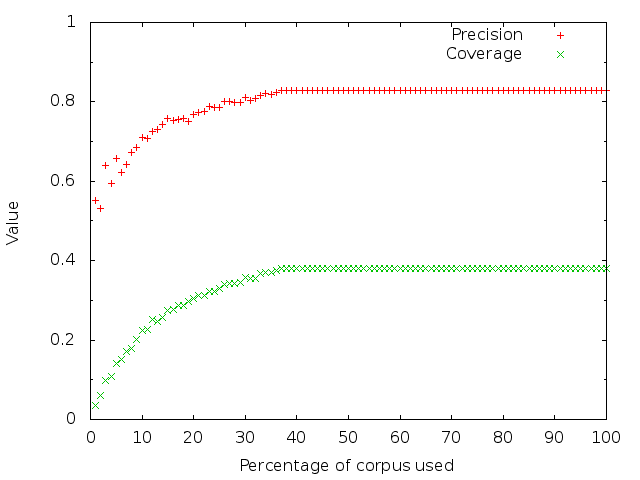
\includegraphics[width=0.45\textwidth]{fig/slot-predicate-percents.png}
    \caption{\label{fig:fonction_predicate}Performance du modèle
        fonction-prédicat en entraînant le modèle sur une sous-partie du corpus
        : de 0 à 100~\%.}
\end{figure}

La figure ~\ref{fig:fonction_predicate} montre que la correspondance
probabiliste a une précision 68.33\% mais une couverture limitée à 38.33\%. Ce
niveau de performance ne demande pas un gros corpus. C'est un enseignement
intéressant pour deux raisons :

\begin{itemize}

    \item Un corpus de petite taille suffit pour obtenir cette performance, ce
    qui est adapté à des domaines où les corpus même non annotés peuvent être
    petits.

    \item L'algorithme ne fait pas de sur-apprentissage en ayant un biais fort
    et une variance faible, ce qui est souhaitable ici.

\end{itemize}

\fi

\subsection{Absence de comparaison avec SEMAFOR}

SEMAFOR \citep{das2014frame} est la référence actuelle en annotation en rôles
sémantiques supervisée : c'est le système qui obtient les meilleurs résultats
sur le corpus full-text de FrameNet 1.5. Sans réussir à relancer nous-même
SEMAFOR\footnote{L'échec d'un collègue rencontré en conférence à utiliser le
code de SEMAFOR et les modèles fournis ne nous a pas encouragé vers cette
voie.} pour s'évaluer sur le même sous-ensemble du corpus FrameNet, une
comparaison directe n'est pas possible :

\begin{itemize}
    \item SEMAFOR annote le corpus FrameNet en frames FrameNet et rôles
        FrameNet alors que nous l'annotons en classes VerbNet et rôles VerbNet
        \textit{seulement quand une corrsepondance existe}.
    \item Toutes les parties du discours sont annotées alors que nous nous
concentrons sur les verbes.
    \item Les tâches sont découpées différemment. En effet, SEMAFOR découpe la
        tâche en trois parties :
    \begin{itemize}
        \item identification des prédicats déclencheurs ;
        \item identification des frames FrameNet ;
        \item identification des arguments et annotation ces arguments avec des
            rôles sémantiques.
    \end{itemize}
\end{itemize}

Nous considérons par la suite uniquement les résultats de SEMAFOR avec
déclencheurs issus de la vérité-terrain : en effet, cette sous-tâche n'est pas
pertinente pour une annotation VerbNet ou PropBank
\citep[section~4]{das2014frame}, et ce n'est de toute façon que sur les
prédicats de la vérité-terrain que nous nous évaluons.

Il est intéressant de noter l'importance des données d'entraînement pour
SEMAFOR : pour l'identification des frames FrameNet les mêmes modèles grimpent
de 74.21~\% à 90.51~\% quand la taille du corpus augmente en passant du corpus
SemEval (2198 phrases) au corpus FrameNet 1.5 (3 256 phrases)
\citep[section~4]{das2014frame}. De la même manière, pour l'identification des
arguments, les résultats augmentent de 46.49~\% à 64.54~\%. C'est très
encourageant pour les domaines disposant de très gros corpus, mais suggère que
d'autres solutions sont à identifier pour les domaines où de tels corpus ne
sont pas disponibles.

\section{Travaux futurs}

Le problème principal est la faible performance de l'identification des
arguments : ce n'était pas là-dessus que nous voulions porter nos efforts, mais
il devient clair que c'est un problème conséquent (section~\ref{resultats_srl})
qui est la priorité pour nos travaux futurs.

Nous pensons aussi prendre en compte la similarité entre les remplisseurs déjà
identifiés et les remplisseurs pour lesquels plusieurs rôles sont possibles
afin d'améliorer nos modèles de probabilité. En effet, l'information des cadres
de sous-catégorisation est cruciale pour identifier les arguments, mais
l'information sémantique concernant le contenu des remplisseurs est aussi utile
pour déterminer le rôle correct, comme nous l'avons vu à la
section~\ref{restrictions_selection}.

Enfin, de la même manière que la prise en compte de la voix passive a amélioré
les résultats, d'autres phénomènes de syntaxe profonde doivent être pris en
compte. La coordination est une autre source commune d'erreur. En effet, quand
deux verbes partagent le même sujet, une analyse syntaxique profonde indique à
chaque fois quel est le sujet profond. Voici deux exemples tirés du corpus
FrameNet :

\begin{itemize}
    \item \textit{You belittle Sheik Bin Baz 's blunder and
        exaggerate the one by Sheik Maqdasi ...}
    \item \textit{Hostile and even friendly nations routinely steal information
        from U.S. companies and share it with their own companies}
\end{itemize}

Dans la première phrase, \textit{you} est détecté comme le sujet du verbe
\textit{belittle}, mais c'est aussi le sujet de \textit{exaggerate}, ce qui
n'est pas détecté. Le problème se pose aussi pour la deuxième phrase
\textit{Hostile and even friendly nations} est le sujet de \textit{share}, ce
qui n'est pas détecté.

Il serait certes possible d'identifier des règles complexes pour traiter ces
cas lors de l'identification des arguments, mais l'objectif est de traiter ces
phénomènes de manière plus générale en intégrant par exemple le système de
\cite{ribeyre2013systeme} qui est conçu pour ce genre de problème et permet de
prendre en compte de nouveaux phénomènes en ajoutant de nouvelles règles au
système. Ainsi, les différents phénomènes seront pris en compte de manière
cohérente.

\section*{Conclusion}

Nous avons implémenté un système d'annotation en rôles sémantiques basé sur la
connaissance. Nous avons utilisé des outils et des corpus disponibles
publiquement qui rendent notre travail facilement reproductible et facilitent
le travail de comparaison, maintenant et dans le futur. Nous avons commencé à
améliorer le système initial, montrant son potentiel. L'indépendance de
l'approche par rapport au corpus considéré la rend attractive pour annoter des
domaines ne disposant que de peu ou pas de corpus annotés en rôles sémantiques.

C'est ce que nous explorons dans le chapitre suivant en étudiant la pertinence
de VerbNet face à des domaines spécifiques et variés : football, réchauffement
climatique et informatique.

